\label{sec:TEO_FRAMEWORK}
%%%%%%%%%%%%%%%%%%%%%%%%%%%%%
\subsection{ELECTROMAGNETIC WAVES}
An electromagnetic wave as shown in figure \ref{fig:PolvNPol} can be characterized by its amplitude ($E_o$), frequency ($w$), phase ($\phi$), direction of the wave ($\Vec{k}$) but also the direction of displacement ($\Vec{P}$). Note that these last vectors are not the same. The former ($\Vec{k}$) refers to the direction in which the light ray propagates and the latter refers to the direction of oscillation. 

\textbf{Def. Polarization}: The direction of the displacement vector is called the \textit{direction of polarization}. Furthermore the plane on which this vector lives and oscillates is the plane of polarization \cite{guenther2015modern}. 
\begin{figure}[H]
    \centering
    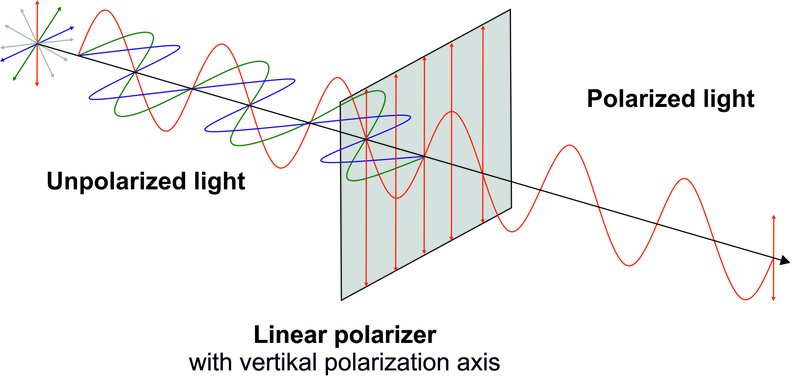
\includegraphics[scale=0.80]{Figures/Polarization_NonPolarization.jpg}
    \caption{Polarized vs Non Polarized light \cite{Pol-figure}}
    \label{fig:PolvNPol}
\end{figure}

\textbf{On the nature of Circular Polarization}\\
A very interesting state of polarization is circular polarization. When we introduce a phase difference equal to $\pi/2$ between the two perpendicular and constituent \footnote{A state of polarization can be mathematically modeled as a vector containing a direction $\hat{x}$ and $\hat{y}$} components of light, the resulting vector of polarization ($\Vec{P}$) propagates in time and space in one of two ways: (i) circular orbits if the components have the same amplitudes or (ii) elliptical orbits if there exists a difference between the components amplitudes. Figure \ref{fig:CircularPol} illustrates this state.

\begin{figure}[H]
    \centering
    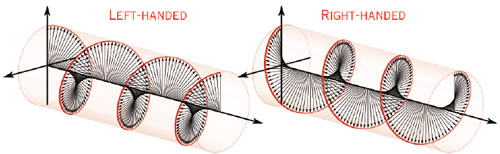
\includegraphics[scale=0.40]{Figures/Circular_Polarization.jpg}
    \caption{Circular Polarization Illustration (N.A)}
    \label{fig:CircularPol}
\end{figure}

One of the biggest misconceptions about this state of polarization is that at any given instant, the polarization state is a circle. Truth is that circular polarization is an emergent illusion that is due to the perpendicular components oscillating out of phase by exactly $pi/2$. This quantity can also be related to the wavelength of the beam. For this case this relation is $\lambda/4$.

%%%%%%%%%%%%%%%%%%%%%%%%%%%%%
\subsection{OPTICAL ELEMENTS}
The main elements for characterizing the polarization of a beam are presented in this section. \\

\textbf{Def. Polarizer:} A polarizer is an optical element that only allows one direction of polarization to be transmitted. For instance, a diagonal polarization incident on a vertical polarization will lose its horizontal component and the transmitted wave will be vertical. \\


\textbf{Def. Retarder:} This type of plate has two different refraction indices on its main perpendicular axis. The axis with a smaller refractive index ($n_f$) will be the fast axis, the other axis with $n_s$ will be the slow axis. Both refractive indices relate to the thickness ($d$) of the element by the relation
\begin{equation}
    d = \frac{\lambda}{4(n_s-n_f)}.
    \label{eq:retard}
\end{equation}
Equation \ref{eq:retard} states a retarder is dependent on the wavelength ($\lambda$) of the beam that is incident. The other key takeaway is that these elements introduce a difference in phase on the components of the light by allowing one component to move fast and the other slow. We will refer to this difference in phase as $\psi$ when we present the experimental results.  


%%%%%%%%%%%%%%%%%%%%%%%%%%%%%
\subsection{MALUS LAW}
Mauls Law is a straight forward mathematical derivation of the power or intensity of a polarized light ray as the polarizer rotates along the optical axis a given angle $\theta$. The relation

\begin{equation*}
    I_{tot} = I_{max}*cos(\theta),
\end{equation*}
is a power full tool to determine a certain state of polarization by measuring the intensity experimentally with previous knowledge of the maximum value $I_{max}$.

%%%%%%%%%%%%%%%%%%%%%%%%%%%%%
\subsection{STOKES PARAMETERS}
The stokes parameters yield information about the polarization state of a particular beam of light. Furthermore, they can be measured in experiments an hence serve as a practical tool that helps when characterizing optical systems. The parameters are the following: 
\\
\begin{enumerate}
    \item $S_0 = |E_x|^2 + |E_y|^2 $\\
    Total power density
    \item $S_1= |E_x|^2 - |E_y|^2 $ 
    Difference between power density transmitted by 2 perpendicular directions of polarization; horizontal and vertical.
    \item $S_2= |E_d|^2 - |E_ad|^2$ 
    Difference between power density transmitted by 2 perpendicular directions of polarization; diagonal and anti-diagonal.
    \item $S_3= |E_R|^2 - |E_L|^2$ 
    Difference between power density transmitted by 2 perpendicular directions of polarization; circular right and left. 
\end{enumerate}

A more elegant way of visualizing such parameters is with a Poincare Sphere (Figure \ref{fig:Poincare}). In this phase space, each axes represent a possible polarized state. A vector within this sphere is a possible polarization state for light. 
\begin{figure}[H]
    \centering
    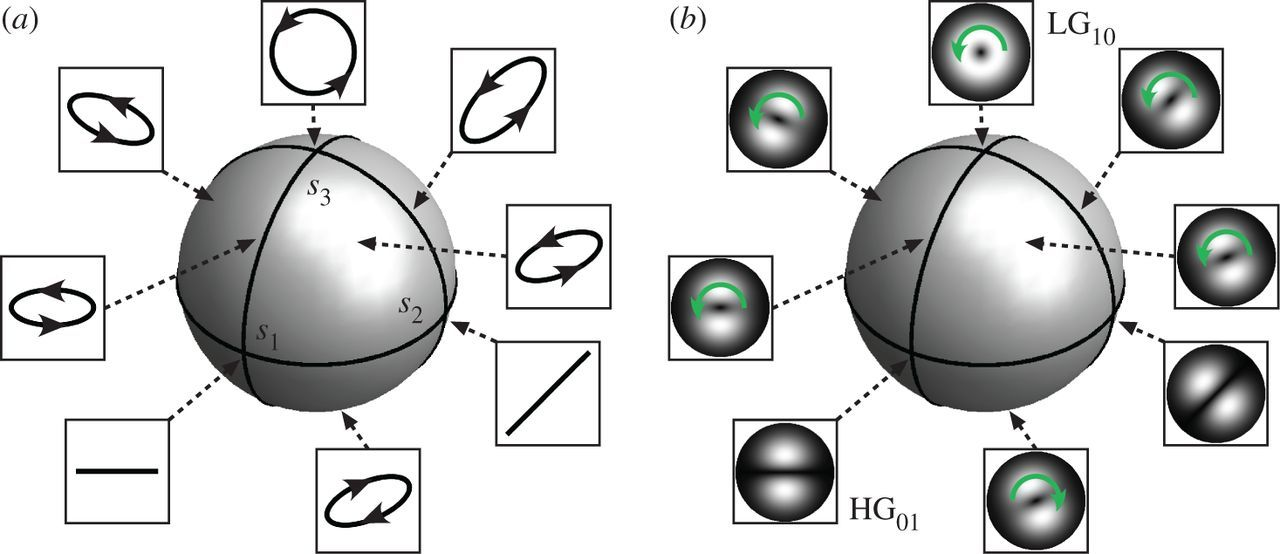
\includegraphics[scale=0.70]{Figures/Poincare.jpg}
    \caption{Poincare Sphere \cite{figpoincare}}
    \label{fig:Poincare}
\end{figure}

